\documentclass[letterpaper,12pt]{article}

% Preamble
\usepackage[utf8]{inputenc}
\usepackage{amsmath, amssymb}
\usepackage{graphicx}
\usepackage{float}
\usepackage{hyperref}
\usepackage{subcaption}
\usepackage{xcolor, soul}
\usepackage{bm}
\usepackage{svg}

\usepackage[style=chem-acs]{biblatex}
\addbibresource{references.bib}
\usepackage{geometry}
\geometry{letterpaper, margin=1in}

\usepackage{tikz}
% \usetikzlibrary{arrows.meta, positioning}  % Load arrows.meta for 'latex' arrow tip

\usepackage{setspace}

\usepackage{titlesec}
\titleformat{\subsubsection}{\normalfont\normalsize}{\thesubsubsection}{1em}{}

\usepackage{caption}
\renewcommand{\figurename}{\textbf{\uppercase{Figure}}}
\renewcommand{\thefigure}{\arabic{figure}}
\captionsetup[figure]{
  labelsep=colon,
  labelfont={bf,small}, % Make label bold in caption
  textfont={small}, % Text in caption remains unbolded and small
  labelformat=default
  }
  \makeatletter
  \let\oldthefigure\thefigure
  \renewcommand{\thefigure}{\arabic{figure}}
  \makeatother
  
  
  \captionsetup[subfigure]{
    labelformat=parens,       % Add parentheses around the label
    labelsep=space,           % Add a space between the label and the caption
    textfont=normalfont,      % Use normal font for the caption text
    position=bottom,          % Position the label at the bottom of the subfigure
    % labelformat=simple,       % Use a simple format without automatic parentheses
    format=plain              % Plain format for subfigure captions
    }
\renewcommand\thesubfigure{\Alph{subfigure}}


\usepackage{multicol}


% Title and author information
\title{Optimal control of axial dispersion tubular reactors with recycle: Addressing state-delay through transport PDEs}
\author{
  Behrad Moadeli \thanks{Department of Chemical and Materials Engineering, University of Alberta, Edmonton, Alberta, Canada, T6G 1H9} \thanks{Corresponding author. Email: moadeil@ualberta.ca} \and
  Guilherme Ozorio Cassol\footnotemark[1] \and
  Stevan Dubljevic \footnotemark[1] 
  }
  
\date{\today}

\begin{document}

\maketitle

\begin{figure}[htbp!]
  \centering
  \includegraphics*[width=0.9\textwidth]{Figures/abstract_final.PNG}
  \caption*{\textbf{Graphical abstract:}
  The boundary-regulated distributed parameter system of an axial dispersion tubular reactor with delayed recycle is showcased, along with the optimal observer-based control strategy developed using a late-lumping method for its stabilization.}
\end{figure}

\newpage
\begin{abstract}
  % Your abstract here
  The optimal control of an axial tubular reactor with a recycle stream is addressed as a key type of setting for of distributed parameter systems in chemical engineering. The intrinsic time delay from the recycle process, thus far overlooked in relevant literature, is modeled as a transport partial differential equation (PDE), resulting in a system of coupled parabolic and hyperbolic PDEs. Utilizing Danckwerts boundary conditions, the reactor is boundary-controlled with the control input at the inlet. A continuous-time optimal linear quadratic regulator is developed to stabilize infinite-dimensional system, employing a late lumping approach in order to preserve the properties of the original infinite dimensional system in controller design. The full-state feedback regulator is designed by solving the Operator Riccati Equation (ORE), leveraging the system's Riesz-spectral properties. To address practical limitations of full-state feedback, a Luenberger observer is also proposed, enabling state reconstruction from boundary measurements. 
  Numerical simulations are conducted to evaluate the proposed control strategies. The results demonstrate that the full-state feedback regulator effectively stabilizes the system. A comparison is made between two configurations where different numbers of eigenmodes were selected to design the controller. The observer-based regulator successfully stabilizes the system using merely output measurements, effectively overcoming the challenge of limited state access.
\end{abstract}

\newpage
% \tableofcontents
% \newpage
      
\onehalfspacing
% \begin{multicols}{2}

  Many chemical, petrochemical, and biochemical unit operation processes are modelled as distributed parameter systems (DPS). When these processes are described using first-principle modeling, they result in a class of partial differential equations (PDEs) to effectively capture diffusion, transport, and reaction phenomena, leading to infinite-dimensional state space representations \autocite{ray1981advanced}. This characteristic presents significant challenges, making the control and estimation of DPS inherently more complex than finite-dimensional systems. Two primary methods have emerged for addressing DPS control. One is early lumping, which approximates the infinite-dimensional system with a finite-dimensional model \autocite{davison1976robust, francis1977linear}. While this method enables the use of standard regulator design techniques, mismatches between the dynamical properties of the original DPS and the approximate lumped parameter model can occur, negatively affecting the performance of the designed regulator \autocite{moghadam2012infinite}. The second method is late lumping, which directly tackles the infinite-dimensional system before applying numerical solutions. This approach introduces a challenging yet fertile direction of research, leading to many meaningful contributions that address various aspects of control and estimation of infinite-dimensional systems.

Among notable studies utilizing late lumping method for control of convection-reaction chemical systems resulting in first order hyperbolic PDEs, \Citeauthor{christofides1998robust} explored the robust control of quasi-linear first-order hyperbolic PDEs, providing explicit controller synthesis formulas for uncertainty decoupling and attenuation \autocite{christofides1998robust}. \Citeauthor{krstic2008backstepping} extended boundary feedback stabilization techniques for first-order hyperbolic PDEs using a backstepping method, converting the unstable PDE into a system for finite-time convergence \autocite{krstic2008backstepping}. Relevant applications of reaction-convection systems other than tubular reactors have also been addressed within this field, resulting in regulator/observer design strategies for chemical systems governed by first order hyperbolic PDEs. \Citeauthor{xu2016state} addressed the state feedback regulator problem for a countercurrent heat exchanger system, utilizing an infinite-dimensional approach to ensure that the controlled output tracks a reference signal \autocite{xu2016state}. Xie and Dubljevic \Citeauthor{xie2021discrete} developed a discrete-time output regulator for gas pipeline networks, emphasizing the transformation of continuous-time models into discrete-time systems while preserving essential continuous-time properties \autocite{xie2021discrete}. This work was further extended by \Citeauthor{zhang2023tracking}, who proposed a tracking model predictive control and moving horizon estimation design for pipeline systems, addressing the challenges of state and parameter estimation in an infinite-dimensional chemical system governed by first order hyperbolic PDEs \autocite{zhang2023tracking}. For a similar convection-reaction system, \Citeauthor{zhang2022dynamic} proposed a model predictive control strategy, incorporating a Luenberger observer to achieve output constrained regulation in a system modeled by nonlinear coupled hyperbolic PDEs \autocite{zhang2022dynamic}.

Additionally, diffusion-convection-reaction systems resulting in parabolic PDEs are also addressed in several works. For example, \Citeauthor{Christofides2012book} addressed order reduction methods for diffusion-convection-reaction type of reactors \autocite{Christofides2012book}. \Citeauthor{dubljevic2006predictive2} utilized modal decomposition to capture dominant modes of a DPS to construct a reduced order finite dimensional system, which enables the design of a low dimensional controller for a diffusion-convection-reaction type reactor described by second order parabolic PDEs \autocite{dubljevic2006predictive2}. \Citeauthor{ozorio2019heat} designed and compared the performance of a full-state and output feedback controller for a diffusion-convection heat exchanger system \autocite{ozorio2019heat}. In \Citeauthor{khatibi2021model}'s work, an axial dispersion tubular reactor equipped with recycle stream is considered as a second order parabolic DPS, with a predictive controller being utilized to optimally control the reactor \autocite{khatibi2021model}.  Although the presence of recycle is common in industrial reactor designs, this work is one of the few contributions in this field that addresses a diffusion-convection-reaction system equipped with a recycle stream.

Moreover, continuous-time optimal control design is a well-developed concept for distributed parameter systems, particularly when the system generator is either a self-adjoint operator or can be transformed into one through a proper linear transformation \autocite{morrisbook}. However, there are distributed parameter systems that do not possess this property. Instead, the system generator belongs to the domain of Riesz-spectral operators. Rather than an orthonormal basis for the function-space, these generators introduce a bi-orthonormal set of eigenfunctions as the basis. Optimal controller design for these systems was initially addressed in \Citeauthor{curtainbook} \autocite{curtainbook}. Since then, significant work has been done in this field. For instance, continuous-time optimal control design for a cracking catalytic reactor, another convection-reaction system governed by first-order hyperbolic PDEs, has been achieved by solving an operator Riccati equation (ORE)\autocite{aksikas2009lq}. This work has been further extended to time-varying PDEs of the same class\autocite{aksikas2013optimal}. The same approach has been applied to develop a full-state feedback\autocite{mohammadi2012lq} and output feedback\autocite{aksikas2024spectral} linear quadratic (LQ) optimal regulator for a boundary-controlled convection-reaction system, utilizing the properties of a Riesz-spectral generator for the system.

On top of those dynamic systems that are distributed in space, delay systems are another example of distributed parameter systems \autocite{curtainbook}. Although delay is commonly represented in the form of delay differential equations (DDEs), it can also be modeled as a transport partial differential equation (PDE), which offers advantages in more complex scenarios or when employing alternative norms on infinite-dimensional states. This approach allows for a smoother transition to problems involving more intricate PDE dynamics while maintaining notational consistency \autocite{krstic2009book}. Input/output delay with relevant applications in chemical engineering has been addressed previously in the field of control theory for DPS. For example, time-delayed boundary observation is considered while addressing an output feedback regulator for a tubular reactor \autocite{Guilherme2019ACC}. However, the notion of state-delay (as opposed to delayed-input or delayed-output) seems to be less addressed in this field compared to other relevant fields like signal processing, self-driving cars, or network control theory (NCT). This is probably because not much application in the field of distributed parameter chemical engineering systems can be introduced in the first place. \Citeauthor{ozorio2019heat}'s work is one of the few instances that addressed a delayed-state distributed parameter chemical engineering system \autocite{ozorio2019heat}, where they designed a full-state and output feedback regulator for a system of heat exchangers. The notion of state-delay comes from the time it takes for a stream to leave one pass of the heat exchanger and enter the next pass. As stated previously, not much work is published addressing chemical reactors equipped with recycle as distributed parameter systems. Even in \Citeauthor{khatibi2021model}'s work, the recycle is assumed to be instantanous; a simplifying assumption that does not resonate well with reality. In fact, taking the time it takes for the recycle stream to re-enter the reactor input can be another instance for the rare concept of a delayed state DPS in the field of chemical engineering.

The present work focuses on the control of an axial tubular reactor equipped with a recycle stream, a configuration common in industrial processes but inadequately addressed in the literature. Unlike previous studies that assumed instantaneous recycle, this work incorporates the time delay associated with the recycle stream re-entering the reactor, presenting a rare example of state-delay in the field of chemical engineering DPS. The model comprises a second-order parabolic PDE to capture the diffusion-convection-reaction nature of the reactor, coupled with a first-order hyperbolic PDE to account for the delay. The boundary conditions are chosen as Danckwerts boundary conditions, which are particularly suitable for this type of reactor. The system results in a non-self-adjoint operator, but by utilizing the bi-orthogonal theorem, given that the generator is Riesz-spectral, a full-state feedback optimal LQ regulator is developed, followed by an output feedback regulator. The control strategy is derived by solving an operator Riccati equation (ORE) and employs a late lumping approach. Actuation and observation are conducted at the boundaries, making it a boundary-actuated system involving finite-dimensional dynamics for an infinite-dimensional DPS. The paper is structured as follows:

\begin{itemize}
    \item Section 1: Modeled the delay infinite-dimensional system (DPS) and transformed it into a system of coupled PDEs using the delay-transport approach. Explored system dynamics by examining eigenvalues, the adjoint operator, and the bi-orthogonal basis, followed by an assessment of the open-loop response.
    \item Section 2: Developed the full-state feedback gain by formulating the infinite-time horizon LQ control problem, converting the ORE into matrix Riccati equations (MRE), and studying the resulting closed-loop response.
    \item Section 3: Addressed practical limitations of the proposed full-state feedback mechanism by introducing a Luenberger observer for state reconstruction, followed by the design of an output feedback regulator. The closed-loop response of this regulator was also analyzed.
    \item Section 4: Provided an illustrative numerical example to demonstrate the practical application of the theoretical concepts developed.
\end{itemize}
  
  \section{OPEN-LOOP SYSTEM} \label{sec:model}

\subsection{System model}

\begin{figure}[!htbp]
    \centering
    \begin{tikzpicture}
        \node (pfr) [cylinder, draw, minimum height=3cm, minimum width=1cm, shape aspect=1, shape border rotate=180, cylinder uses custom fill, cylinder end fill=gray!45, cylinder body fill=gray!15] {$\mathcal{A} \rightarrow \mathcal{B}$};
        \node (pfr_inlet) [circle, left of=pfr, xshift=-0.5cm, fill=black, draw, inner sep=0pt, minimum size=0.25cm, scale=0.5] {};
        \node (pfr_outlet) [circle, at={(pfr.east)}, shift={(-0.25cm,0)}, fill=black, draw, inner sep=0pt, minimum size=0.25cm, scale=0.5] {};
        \node (recycle_right) [circle, right of=pfr_outlet, fill=black, draw, inner sep=0pt, minimum size=0.25cm, scale=0.5] {};
        \node (recycle_left) [circle, left of=pfr_inlet, fill=black, draw, inner sep=0pt, minimum size=0.25cm, scale=0.5] {};
    
        \draw[dotted, thick] ([yshift=0.5cm]pfr_inlet.center) -- node[at end, below, yshift=0.1cm] {$\zeta = 0$} ([yshift=-0.65cm]pfr_inlet.center);
        \draw[dotted, thick] ([yshift=0.5cm]pfr_outlet.center) -- node[at end, below, yshift=0.1cm] {$\zeta = 1$} ([yshift=-0.65cm]pfr_outlet.center);
    
        \node[below of=recycle_left, node distance=1.3cm, anchor=north west, xshift=-0.2cm] {$R \, c(1, t-\tau)$};
        \node[above of=pfr_inlet, node distance=0.75cm,] {$c(0, t)$};
        \node[above of=pfr_outlet, node distance=0.75cm,] {$c(1, t)$};
        
        \draw [arrow_2] (pfr_outlet) -- node[near end, above] {$y(t)$} ++(2,0);
        \draw [arrow_2] (pfr_inlet) ++(-2,0) coordinate(start) -- node[near start, above] {$u(t)$} (pfr_inlet);
        \draw [arrow_2] (recycle_right) -- ++(0,-1.25) -| (recycle_left);
        
    \end{tikzpicture}
    \caption{Axial tubular reactor with recycle stream.}
    \label{fig:reactor_scheme}
\end{figure}


The chemical process illustrated in Figure~\ref{fig:reactor_scheme} represents an axial dispersion tubular reactor, which incorporates diffusion, convection, and a first-order irreversible chemical reaction \autocite{levenspiel1998chemical}. The reactor is equipped with a recycle mechanism, allowing a fraction of the product stream to re-enter the reactor to ensure the consumption of any unreacted substrate. By applying first-principle modeling through relevant mass balance relations on an infinitesimally small section of the reactor, the reactor's dynamics can be described by a second-order parabolic PDE, a common class of equations used to characterize diffusion-convection-reaction systems \autocite{jensen1982bifurcation}. The resulting PDE that describes the reactor model is given by:

\begin{equation} \label{eq:PDE_original_model}
    \dot{c}(\zeta, t) = D \partial_{\zeta \zeta} c(\zeta, t) - v \partial_\zeta c(\zeta, t) + k_r c(\zeta, t)
\end{equation}

subject to Dankwerts boundary conditions:

\begin{align} \label{eq:BC}
    \begin{cases}
        &D \partial_\zeta c(0, t) - v c(0, t) = -v \left[ R c(1, t-\tau) + (1-R) u(t) \right] \\
        &\partial_\zeta c(1, t) = 0 \\
        &y(t) = c(1, t)
    \end{cases}
\end{align}

Here, $c(\zeta, t)$ denotes the properly scaled notion of concentration along the reactor, representing the state of the system. The physical parameters $D$, $v$, $k_r$, $R$, and $\tau$ correspond to the diffusion coefficient, flow velocity along the reactor, reaction constant, recycle ratio, and residence time of the recycle stream, respectively. The spatial and temporal coordinates of the system are represented by $\zeta$ and $t$, where $\zeta \in [0, 1]$ and $t \in [0, \infty)$.

Dankwerts boundary conditions are particularly suitable for modeling axial tubular reactors, as they account for deviations from perfect mixing and piston flow, assuming negligible transport lags in connecting lines \autocite{danckwerts1993continuous}. These conditions make the model more realistic for chemical reactors of this type. The input and the output of the system are also present in the boundary conditions. The system output is measured at the reactor outlet, while the input is applied at the inlet. Additionally, the delayed state resulting from the recycled portion of the flow, occurring $\tau$ time units ago, is incorporated into the inlet; all as shown in Equation~(\ref{eq:BC}).


\subsection{PDE representation of delay term}

One effective method for addressing delay in systems is to represent the delay using an alternative transport partial differential equation (PDE). This approach is particularly advantageous when the problem already involves similar forms of PDEs, as is the case in the current study. To specifically address the delay in the system under consideration, the state variable $c(\zeta, t)$ is expanded into a vector of functions $\bm{x}(\zeta, t) \equiv [x_1(\zeta, t), x_2(\zeta, t)]^T$, where $x_1(\zeta, t)$ represents the concentration within the reactor, and $x_2(\zeta, t)$ is introduced as a new state variable to account for the concentration along the recycle stream. The delay is thus modeled as a pure transport process, wherein the first state $x_1(\zeta, t)$ is transported from the reactor outlet to the inlet, experiencing a delay of $\tau$ time units while in the recycle stream. As a result, Equations~\ref{eq:PDE_original_model}~and~\ref{eq:BC} may be re-formulated as follows:

\begin{align}
    \partial_t 
    \begin{bmatrix}
        x_1(\zeta, t) \\ x_2(\zeta,t)
    \end{bmatrix}
    =
    \begin{bmatrix}
        D \partial_{\zeta \zeta} - v \partial_\zeta + k_r && 0 \\
        0 && \frac{1}{\tau} \partial_\zeta
    \end{bmatrix}
    \begin{bmatrix}
        x_1(\zeta, t) \\ x_2(\zeta,t)
    \end{bmatrix}\\
\begin{cases}
    D \partial_\zeta x_1(0, t) - v x_1(0, t) = -v \left[ R x_2(0, t) + (1-R) u(t) \right] \\
    \partial_\zeta x_1(1, t) = 0 \\
    x_1(1,t) = x_2(1,t) \\
    y(t) = x_1(1, t)
\end{cases}
\end{align}

With all state variables now expressed explicitly at a specific time instance $t$—in contrast to the previous representation where states at $t$ were directly involved with states at $(t-\tau)$—the open-loop system can be described in the standard state-space form of an infinite-dimensional linear time-invariant (LTI) system as $\dot{\bm{x}} = \mathfrak{A} \bm{x}$. Here, $\mathfrak{A}$ is a linear operator $\mathcal{L}(X)$ acting on a Hilbert space $X: L^2[0,1] \times L^2[0,1]$ and $\bm{x}(\zeta,t)$, as defined previously, is the vector of functions describing the states of the system. The operator $\mathfrak{A}$ and its domain are defined in detail as shown in Equation~(\ref{eq:operator_A}):

\begin{equation} \label{eq:operator_A}
    \begin{aligned}
        \mathfrak{A} \equiv&
        \begin{bmatrix}
            D \partial_{\zeta \zeta} - v \partial_\zeta + k_r & 0 \\
            0 & \frac{1}{\tau} \partial_\zeta
        \end{bmatrix}\\
        \mathcal{D}(\mathfrak{A}) =& \Bigl\{ \bm{x} = [x_1, x_2]^T \in X:
        \bm{x}(\zeta), \partial_\zeta \bm{x}(\zeta), \partial_{\zeta \zeta} \bm{x}(\zeta) \quad \mathrm{a.c.},\\
        &D \partial_\zeta x_1(0) - v x_1(0) = -v \left[ R x_2(0) + (1-R) u \right],\\
        &\partial_\zeta x_1(1) = 0,
        x_1(1) = x_2(1) \Bigr\}
    \end{aligned}
\end{equation}

\subsection{Adjoint operator}

The adjoint operator $\mathfrak{A}^*$ plays a critical role in analyzing the spectral properties of the system. It is obtained in Equation~(\ref{eq:adjoint_A}):

\begin{equation} \label{eq:adjoint_A}
    \begin{aligned}
        \langle \mathfrak{A} \bm{\phi}, \bm{\psi}\rangle  = \langle \bm{\phi}, {\mathfrak{A}}^{*} \bm{\psi}\rangle  &\Rightarrow \\
        {\mathfrak{A}}^{*} =&
        \begin{bmatrix}
            D \partial_{\zeta \zeta} + v \partial_\zeta +k_r & 0\\
            0 & -\frac{1}{\tau} \partial_\zeta
        \end{bmatrix}\\
        \mathcal{D}(\mathfrak{A}^*) =& \Bigl\{ \bm{y} = [y_1, y_2]^T \in Y:
        \bm{y}(\zeta), \partial_\zeta \bm{y}(\zeta), \partial_{\zeta \zeta} \bm{y}(\zeta) \quad \mathrm{a.c.},\\
        &D \partial_\zeta y_1(1) + v y_1(1) = \frac{1}{\tau} y_2(1) \\
        &R v y_1(0) = \frac{1}{\tau} y_2(0) \\
        &\partial_\zeta y_1(0) = 0 \Bigr\}
    \end{aligned}
\end{equation}

where $\bm{\phi_i}(\zeta) = [\phi_{i,1}(\zeta), \phi_{i,2}(\zeta)]^T$ and $\bm{\psi_i}(\zeta) = [\psi_{i,1}(\zeta), \psi_{i,2}(\zeta)]^T$ are the eigenfunction of $\mathfrak{A}$ and $\mathfrak{A}^*$, respectively. Given that $\mathfrak{A}$ is not self-adjoint (i.e., $\mathfrak{A} \neq \mathfrak{A}^*$), their combined eigenmodes may still form a bi-orthonormal basis, typical of a Riesz-spectral operator \autocite{curtainbook}. Therefore their spectral properties must be determined by solving their characteristic equations.

\subsection{Eigenvalue problem}

The eigenvalue problem for $\mathfrak{A}$ is formulated as:

\begin{equation} \label{eq:eig_prob}
        \mathfrak{A} \bm{\phi_i}(\zeta) = \lambda_i \bm{\phi_i}(\zeta)
\end{equation}


where $\lambda_i \in \mathbb{C}$ is the $i^{\text{th}}$ eigenvalue. To obtain the characteristic equation, the system of PDEs shall be reduced to the ODE system in Equation~(\ref{eq:eigval_calc_2}) $\forall i \geq 0$:

\begin{equation} \label{eq:eigval_calc_2}
    \begin{aligned}
        \partial_\zeta \begin{bmatrix}
            \phi_1 \\ \partial_\zeta \phi_1 \\ \phi_2
        \end{bmatrix} = \begin{bmatrix}
            0 & 1 & 0 \\
            \frac{\lambda-k_r}{D} & \frac{v}{D} & 0 \\
            0 & 0 & \tau \lambda 
        \end{bmatrix} \begin{bmatrix}
            \phi_1 \\ \partial_\zeta \phi_1 \\ \phi_2
        \end{bmatrix}
    \end{aligned}
\end{equation}

which is in the form of $ \tilde{\bm{\phi}}_\zeta  = \tilde{\mathfrak{A}} \tilde{\bm{\phi}}$, with the solution stated in Equation~(\ref{eq:eigval_calc_3}):

\begin{equation} \label{eq:eigval_calc_3}
    \begin{bmatrix}
        \phi_1 \\ \partial_\zeta \phi_1 \\ \phi_2
    \end{bmatrix}_{\zeta=1} = \begin{bmatrix}
        \Lambda_{1,1} & \Lambda_{1,2} & \Lambda_{1,3} \\
        \Lambda_{2,1} & \Lambda_{2,2} & \Lambda_{2,3} \\
        \Lambda_{3,1} & \Lambda_{3,2} & \Lambda_{3,3}
    \end{bmatrix} \begin{bmatrix}
        \phi_1 \\ \partial_\zeta \phi_1 \\ \phi_2
    \end{bmatrix}_{\zeta=0}
\end{equation}

where the $ 3 \times 3$ matrix $\Lambda_{(m,n)}$ is defined as $\Lambda \equiv \left. e^{\tilde{\mathfrak{A}} (\zeta - 0)} \right|_{\zeta = 1}$. By applying the boundary conditions to Equation~(\ref{eq:eigval_calc_3}), the algebraic system of equations in Equation~(\ref{eq:eigval_calc_4}) is obtained:

\begin{equation} \label{eq:eigval_calc_4}
    \begin{bmatrix}
        -v & D & Rv \\
        \Lambda_{2,1} & \Lambda_{2,2} & \Lambda_{2,3} \\
        (\Lambda_{1,1} - \Lambda_{3,1}) & (\Lambda_{1,2} - \Lambda_{3,2}) & (\Lambda_{1,3} - \Lambda_{3,3})
    \end{bmatrix} \begin{bmatrix}
        \phi_1 \\ \partial_\zeta \phi_1 \\ \phi_2
    \end{bmatrix}_{\zeta=0} = \tilde{\Lambda} \left. \tilde{\bm{\phi}} \right|_{\zeta = 0} = 0
\end{equation}

where $\tilde{\Lambda}$ is defined as the square matrix shown in Equation~(\ref{eq:eigval_calc_4}). Equation~(\ref{eq:eigval_calc_4}) suggests that the matrix $\tilde{\Lambda}$ must be rank-deficient for appropriate values of $\lambda_i$. Attempts to analytically solve the characteristic equation $det(\tilde{\Lambda}) = 0$ has failed; therefore, it is solved numerically using the parameters in Table~\ref{tab:pars}. The resulting eigenvalue distribution is depicted in Figure~\ref{fig:eigval_dist} in the complex plane.

\begin{figure}[!htbp]
    \centering
    \includesvg[inkscapelatex=false, width=0.8\textwidth, keepaspectratio]{Figures/eig_val_dist_R_0.3.svg}
    \caption{Eigenvalues of operator $\mathfrak{A}$ obtained by solving Equation~(\ref{eq:eigval_calc_4}).}
    \label{fig:eigval_dist}
\end{figure}


\begin{table}[ht]
    \centering
    \caption{Physical Parameters for the System}
    \label{tab:pars}
    \begin{tabular}{|c|c|c|c|}
    \hline
    \textbf{Parameter}        & \textbf{Symbol} & \textbf{Value}     & \textbf{Unit}    \\ \hline
    Diffusivity               & $D$             & $2\times10^{-5}$   & ${m^2}/{s}$      \\ \hline
    Velocity                  & $v$             & $0.01$   & ${m}/{s}$        \\ \hline
    Reaction Constant         & $k_r$           & $1.5$              & $s^{-1}$         \\ \hline
    Recycle Residence Time    & $\tau$          & $80$               & $s$              \\ \hline
    Recycle Ratio             & $R$             & $0.3$              & $-$              \\ \hline
    \end{tabular}
\end{table}

Following the same procedure for $\mathfrak{A}^*$ shows that the eigenvalues of $\mathfrak{A}$ match the ones of its adjoint, confirming that $\mathfrak{A}$ and $\mathfrak{A}^*$ form a bi-orthogonal basis according to Equation~(\ref{eq:biorth}):

\begin{equation} \label{eq:biorth}
    \begin{aligned}
        &\langle \mathfrak{A} \bm{\phi_i}, \bm{\psi_j} \rangle = \langle \lambda_i \bm{\phi_i}, \bm{\psi_j} \rangle = \lambda_i \langle \bm{\phi_i}, \bm{\psi_j} \rangle \\
        \text{L.H.S.} = &\langle \bm{\phi_i}, \mathfrak{A}^* \bm{\psi_j} \rangle = \langle \bm{\phi_i}, \lambda_j^* \bm{\psi_j} \rangle = \overline{\lambda_j^*} \langle \bm{\phi_i}, \bm{\psi_j} \rangle \\
        &\lambda_i = \overline{\lambda_i^*} \Rightarrow \langle \bm{\phi_i}, \bm{\psi_j} \rangle = \delta_{ij}
    \end{aligned}
\end{equation}

The eigenfunctions $\{ \bm{\phi_i}(\zeta), \bm{\psi_i}(\zeta) \}$ (for $\mathfrak{A}$ and $\mathfrak{A}^*$, respectively) may be obtained following the calculation of eigenvalues. The first 3 eigenfunctions are plotted in Figure~\ref{fig:eigfun}. 

\begin{figure}[H]
    \centering
    \includesvg[inkscapelatex=false, width=0.6\textwidth, keepaspectratio]{Figures/eigfuns.svg}
    \caption{First few eigenmodes of $\mathfrak{A}$ and $\mathfrak{A}^*$.}
    \label{fig:eigfun}
\end{figure}

  
  \input{Sections/03_control.tex}
    
  \section{NUMERICAL EVALUATION OF SYSTEM DYNAMICS}

The obtained controller strategies in the previous section are applied to a finite-difference method (FDM) representation of the system model to evaluate the system dynamics. The system model is discretized in space and time, and the resulting system of ordinary differential equations is solved using the \texttt{`solve\_ivp'} function in Python's \texttt{`SciPy'} library \autocite{2020SciPy}, which employs the adaptive Runge-Kutta method of order 5(4), \texttt{`RK45'}. Each state of the system is discretized in space using 100 grid points. The \texttt{`RK45'} method automatically adjusts time steps to balance accuracy and computational efficiency, with the solution being evaluated at specific points as required. First, the unstable dynamics of the open-loop system is explored. Then two full-state feedback systems are compared with respect to number of eigenmodes used to obtain the optimal feedback gain. Finally, the performance of the proposed observer-based controller is evaluated and the state reconstruction error dynamics are analyzed.

\subsection{FDM representation of the open-loop system}

Zero-input response of the system is first explored using a finite-difference method (FDM) representation to show the unstable dynamics of the model. The state profile versus time and space is illustrated in Figure~\ref{ig:3D_x1_openloop}. The goal is to stabilize the system using an optimal control strategy.

\begin{figure}[H]
    \centering
    \includegraphics[width=0.8\textwidth]{Figures/3D_x1_openloop.png}
    \caption{3D plot of the open-loop system}
    \label{fig:3D_x1_openloop}
\end{figure}

\subsection{Full-state feedback regulator FDM representation}

\textbf{add improvement in cost function. Done}

\begin{equation*}
    10 percent from 1 to 3. less than 1 percent from 3 to 7. changes with Q, R, N_{zeta}, but insignificant
\end{equation*}


Next, the full-state feedback regulator is evaluated using an FDM representation. Two configurations are compared: one with $N=3$ eigenmodes and another with $N=7$ eigenmodes. Figures \ref{fig:3D_x1_k3} and \ref{fig:3D_x1_k7} show the 3D plots of the system dynamics for these configurations. The 2D plot in Figure \ref{fig:2D_xt_k7} provides a detailed view of the state trajectories for the $N=7$ configuration.

\begin{figure}[H]
    \centering
    \begin{subfigure}[b]{0.45\textwidth}
        \includegraphics[width=\textwidth]{Figures/3D_x1_k3.png}
        \caption{Full-state feedback regulator with $N=3$}
        \label{fig:3D_x1_k3}
    \end{subfigure}
    \hfill
    \begin{subfigure}[b]{0.45\textwidth}
        \includegraphics[width=\textwidth]{Figures/3D_x1_k7.png}
        \caption{Full-state feedback regulator with $N=7$}
        \label{fig:3D_x1_k7}
    \end{subfigure}
    \caption{FDM representation of the full-state feedback regulator}
    \label{fig:full_state_feedback}
\end{figure}

\begin{figure}[H]
    \centering
    \includegraphics[width=0.8\textwidth]{Figures/2D_xt_k7.png}
    \caption{2D plot of the full-state feedback regulator with $N=7$}
    \label{fig:2D_xt_k7}
\end{figure}

\subsection{Observer-based regulator FDM representation}

Finally, the observer-based regulator is evaluated using an FDM representation. The system model is discretized in space and time, and the resulting system of ordinary differential equations is solved using the \texttt{solve\_ivp} function in Python. Figures \ref{fig:3D_x1_L_k7} and \ref{fig:2D_xt_L_k7} show the 3D and 2D plots of the observer-based regulator, respectively. The error dynamics of the observer-based regulator are illustrated in Figures \ref{fig:3D_e1_L_k7} and \ref{fig:2D_et_L_k7}, providing insights into the state reconstruction error over time.

\begin{figure}[H]
    \centering
    \includegraphics[width=0.8\textwidth]{Figures/3D_x1_L_k7.png}
    \caption{3D plot of the observer-based regulator}
    \label{fig:3D_x1_L_k7}
\end{figure}

\begin{figure}[H]
    \centering
    \includegraphics[width=0.8\textwidth]{Figures/2D_xt_L_k7.png}
    \caption{2D plot of the observer-based regulator}
    \label{fig:2D_xt_L_k7}
\end{figure}

\begin{figure}[H]
    \centering
    \includegraphics[width=0.8\textwidth]{Figures/3D_e1_L_k7.png}
    \caption{3D plot of the error dynamics of the observer-based regulator}
    \label{fig:3D_e1_L_k7}
\end{figure}

\begin{figure}[H]
    \centering
    \includegraphics[width=0.8\textwidth]{Figures/2D_et_L_k7.png}
    \caption{2D plot of the error dynamics of the observer-based regulator}
    \label{fig:2D_et_L_k7}
\end{figure}

  \input{Sections/05_conc.tex}
  
  \newpage
  \printbibliography

  % \end{multicols}

\newpage
\section*{FIGURES}

\begin{figure}[!htbp]
    \centering
    \includegraphics[width=0.7\textwidth]{Figures/sample.jpeg}
    \caption{Sample figure.}
    \label{fig:reactor_scheme}
\end{figure}

\begin{figure}[!htbp]
    \centering
    \includegraphics[width=0.7\textwidth]{Figures/eigval_dist_R_0.3.jpg}
    \caption{Eigenvalues of operator $\mathfrak{A}$ plotted on complex plane}
    \label{fig:eigval_dist}
\end{figure}

\begin{figure}[!htbp]
    \centering
    \includegraphics[width=0.7\textwidth]{Figures/eigfuns.png}
    \caption{First few eigenmodes of $\mathfrak{A}$ and $\mathfrak{A}^*$}
    \label{fig:eigfun}
\end{figure}

\begin{figure}[!htbp]
    \centering
    \begin{subfigure}[b]{0.45\textwidth}
        \centering
        \includegraphics[width=\textwidth]{Figures/k_3.png}
        \caption{$N = 3$}
        \label{fig:k_3}
    \end{subfigure}
    \hfill
    \begin{subfigure}[b]{0.45\textwidth}
        \centering
        \includegraphics[width=\textwidth]{Figures/k_7.png}
        \caption{$N = 7$}
        \label{fig:k_7}
    \end{subfigure}
    \caption{Full-state feedback gain $K(\zeta)$ utilizing the first 7 modes of the system.}
    \label{fig:k_modes}
\end{figure}

\begin{figure}[!htbp]
    \centering
    \includegraphics*[width=0.7\textwidth]{Figures/sample.jpeg}
    \caption{Block diagram representation of the full-state feedback control system.}
    \label{fig:block_diagram}
\end{figure}

\begin{figure}[!htbp]
    \centering
    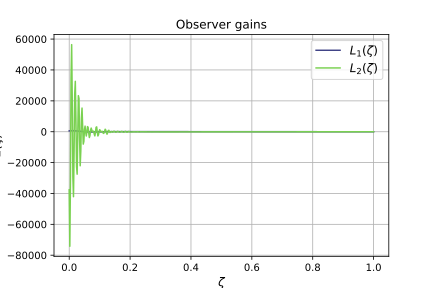
\includegraphics[width=0.7\textwidth]{Figures/L.png}
    \caption{Observer gain $L(\zeta)$.}
    \label{fig:L_modes}
\end{figure}

\begin{figure}[!htbp]
    \centering
    \includegraphics*[width=0.7\textwidth]{Figures/pole_placement.png}
    \caption{Eigenvalues of the observer-based controller, full-state feedback controller, and open-loop system.}
    \label{fig:eigs}
\end{figure}

\begin{figure}[!htbp]
    \centering
    \includegraphics*[width=0.7\textwidth]{Figures/sample.jpeg}
    \caption{Block diagram representation of the full-state feedback control system.}
    \label{fig:block_diagram_observer}
\end{figure}

\begin{figure}[!htbp]
    \centering
    \includegraphics[width=0.8\textwidth]{Figures/3D_x1_openloop.png}
    \caption{3D plot of the open-loop system}
    \label{fig:3D_x1_openloop}
\end{figure}

\begin{figure}[!htbp]
    \centering
    \begin{subfigure}[b]{0.45\textwidth}
        \includegraphics[width=\textwidth]{Figures/3D_x1_k3.png}
        \caption{Full-state feedback regulator with $N=3$}
        \label{fig:3D_x1_k3}
    \end{subfigure}
    \hfill
    \begin{subfigure}[b]{0.45\textwidth}
        \includegraphics[width=\textwidth]{Figures/3D_x1_k7.png}
        \caption{Full-state feedback regulator with $N=7$}
        \label{fig:3D_x1_k7}
    \end{subfigure}
    \caption{FDM representation of the full-state feedback regulator}
    \label{fig:full_state_feedback}
\end{figure}

\begin{figure}[!htbp]
    \centering
    \includegraphics[width=0.8\textwidth]{Figures/2D_xt_k7.png}
    \caption{2D plot of the full-state feedback regulator with $N=7$}
    \label{fig:2D_xt_k7}
\end{figure}

\begin{figure}[!htbp]
    \centering
    \includegraphics[width=0.8\textwidth]{Figures/3D_x1_L_k7.png}
    \caption{3D plot of the observer-based regulator}
    \label{fig:3D_x1_L_k7}
\end{figure}

\begin{figure}[!htbp]
    \centering
    \includegraphics[width=0.8\textwidth]{Figures/2D_xt_L_k7.png}
    \caption{2D plot of the observer-based regulator}
    \label{fig:2D_xt_L_k7}
\end{figure}

\begin{figure}[!htbp]
    \centering
    \includegraphics[width=0.8\textwidth]{Figures/3D_e1_L_k7.png}
    \caption{3D plot of the error dynamics of the observer-based regulator}
    \label{fig:3D_e1_L_k7}
\end{figure}

\begin{figure}[!htbp]
    \centering
    \includegraphics[width=0.8\textwidth]{Figures/2D_et_L_k7.png}
    \caption{2D plot of the error dynamics of the observer-based regulator}
    \label{fig:2D_et_L_k7}
\end{figure}


% \newpage

% \begin{equation}
%   \begin{align}
%     u(t) &\qquad \qquad x(0, t) \\
%     y(t) &\qquad \qquad x(1, t) \\
%     \zeta = 0 &\qquad \qquad \zeta = 1 \\
%     R x(1, t - \tau) &\qquad \qquad \hat{x}(\zeta,t) \\
%     \mathcal{A} \rightarrow \mathcal{B} \\
%   \end{align}
% \end{equation}

\end{document}
